% !TEX root = ../main.tex
\section{Physical Regimes of the Mean-Force State}
\label{sec:response_scale}\label{sec:numerical_v6}

The exact qubit solution isolates a single scalar control variable,
\(\chi\), so it is natural to organize the state diagnostics around it.
Reintroducing an explicit dimensionless coupling strength through
\begin{equation}
    K(u)=g^2 K_0(u),
\end{equation}
all response kernels inherit the same quadratic scaling and the influence
magnitude factorizes as
\begin{equation}
    \chi(\beta,g,\theta)=g^2\chi_0(\beta,\theta).
\end{equation}
The entire recombination of bare Gibbs weight and bath influence is therefore
controlled by the universal scalar function
\begin{equation}
    \gamma(\chi)=\frac{\tanh\chi}{\chi}.
    \label{eq:gamma_chi_crossover_v5}
\end{equation}

The exact crossover scale is determined by \(\chi\sim 1\), or equivalently
\begin{equation}
    \chi(\beta,g,\theta)\sim 1
    \qquad \Longleftrightarrow \qquad
    g^2 \sim \chi_0(\beta,\theta)^{-1},
    \label{eq:chi_crossover_condition_v5}
\end{equation}
which defines the coupling scale
\begin{equation}
    g_\star(\beta)=\chi_0(\beta,\theta)^{-1/2}.
    \label{eq:gstar_def_v6}
\end{equation}
No approximation has been made here: \(g_\star(\beta)\) is an exact property of
the reduced generator.

Two benchmark asymptotes remain useful. For \(\chi\ll 1\),
\begin{equation}
    \gamma(\chi)\simeq 1-\frac{\chi^2}{3},
    \label{eq:gamma_weak}
\end{equation}
so the reduced state tracks the bare Gibbs description with perturbative
bath-induced corrections. For \(\chi\gg 1\),
\begin{equation}
    \gamma(\chi)\simeq \chi^{-1},
    \label{eq:gamma_strong}
\end{equation}
so the reduced generator is dominated by the normalized influence direction.
These asymptotes are best read as benchmarks. The main point is that the full
crossover is captured by one response coordinate.

To make these statements concrete we choose the windowed Ohmic spectral density
\begin{equation}
  J(\omega) = g^2\,\omega\,e^{-\omega/\omega_c},
  \qquad \omega\in[0, 2\omega_q],
  \label{eq:J_ohmic_v6}
\end{equation}
with cutoff \(\omega_c=5\omega_q\). The ultraviolet window matches the
finite-mode simulations of the next section, while the exponential cutoff
regularizes the high-frequency tail~\cite{nematiCouplingFunctionBath2022a}.
Having fixed the bath, we set \(\theta=\pi/4\) and \(\omega_q=1\), since the
remaining behavior is already captured by the universal \(\chi\)-scaling.

\begin{figure}[t]
  \centering
  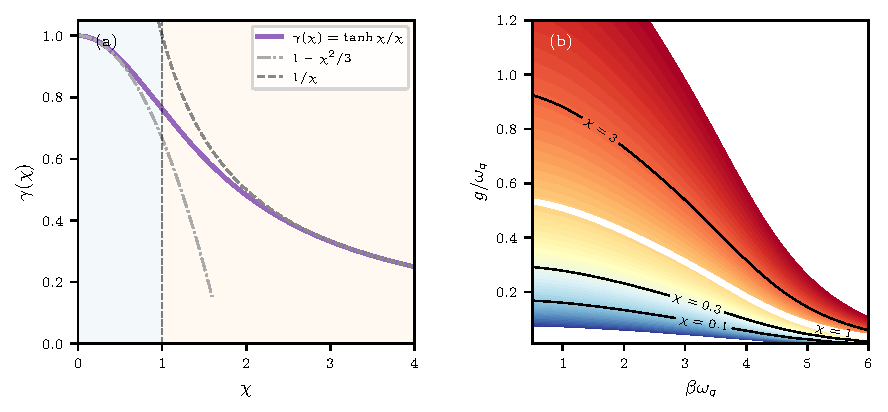
\includegraphics[width=0.48\textwidth]{../figures/hmf_fig1_chi_theory_ab.pdf}
  \caption{Universal crossover structure for the exact qubit mean-force state.
    \textit{Panel~(a)}: Recombination function
    \(\gamma(\chi)=\tanh\chi/\chi\), which interpolates between the small-\(\chi\)
    and large-\(\chi\) benchmarks and makes the \(\chi\sim 1\) crossover
    explicit.
    \textit{Panel~(b)}: Contour map of \(\chi(\beta,g)=g^2\chi_0(\beta)\) for
    the Ohmic bath \eqref{eq:J_ohmic_v6}. The highlighted locus \(\chi=1\)
    defines the exact crossover scale \(g_\star(\beta)=\chi_0(\beta)^{-1/2}\),
    separating weak-response and strongly dressed sectors.}
  \label{fig:chi_theory}
\end{figure}

The same scale organizes the state geometry itself. For a qubit,
\begin{equation}
  \mathcal P_Q = \frac{1}{2}(1+r_Q^2),
\end{equation}
so the Bloch radius \(r_Q\) directly measures the purity of the reduced
equilibrium state. In the exact solution, increasing coupling drives the state
away from the bare thermal radius
\(r_0=\tanh(\beta\omega_q/2)\) and toward a more strongly dressed state. The
effect is most visible at high temperature, where the bare Gibbs state is
nearly mixed and bath-induced structure is easiest to see.

\begin{figure}[t]
  \centering
  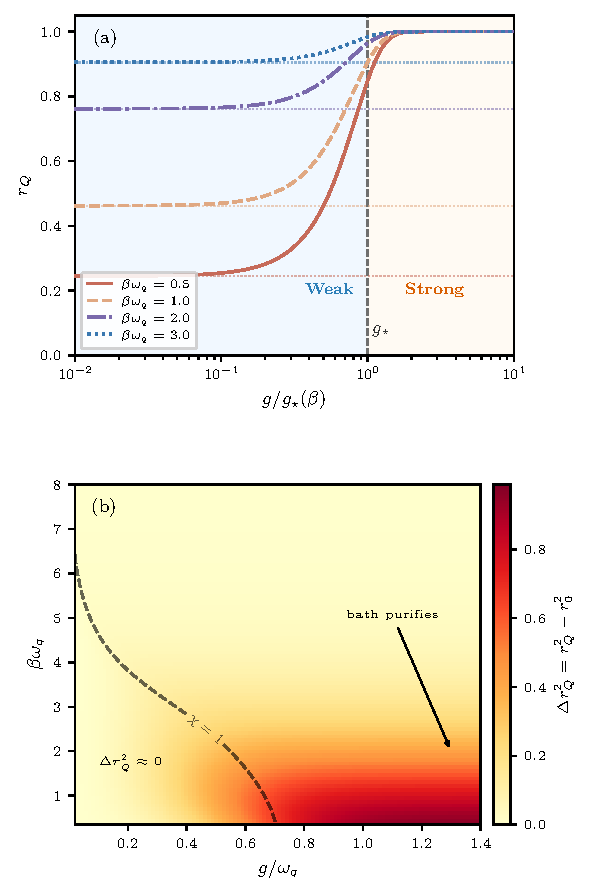
\includegraphics[width=\columnwidth]{../figures/hmf_purity_figure.pdf}
  \caption{Purification diagnostics for the exact qubit mean-force state.
    \textit{Panel~(a)}: Reduced-state Bloch radius \(r_Q\) versus scaled
    coupling \(g/g_\star(\beta)\) for several temperatures. Dotted horizontal
    lines mark the corresponding bare thermal radii \(r_0\); the dressed state
    moves away from the bare Gibbs value most sharply near the crossover.
    \textit{Panel~(b)}: Purity excess
    \(\Delta r_Q^2 \equiv r_Q^2-r_0^2\) over the \((g,\beta)\) plane. The
    dashed contour \(\chi=1\) tracks the same crossover scale seen in
    Fig.~\ref{fig:chi_theory}.}
  \label{fig:purity_figure}
\end{figure}

The same coordinate also controls how rapidly the reduced state changes.
Differentiating the exact Bloch components shows that the angle susceptibility
and radius gradient peak at fixed values of \(\chi\), namely
\(\chi_{\mathrm{peak},\varphi}\approx 0.42\) and
\(\chi_{\mathrm{peak},r}\approx 0.85\) for the Ohmic example used below. After
rescaling the coupling as \(g/g_\star(\beta)\), these peaks align across
temperatures. The alignment is not a numerical accident; it is the statement
that the response scale is intrinsic to the exact reduced generator.

\begin{figure}[t]
  \centering
  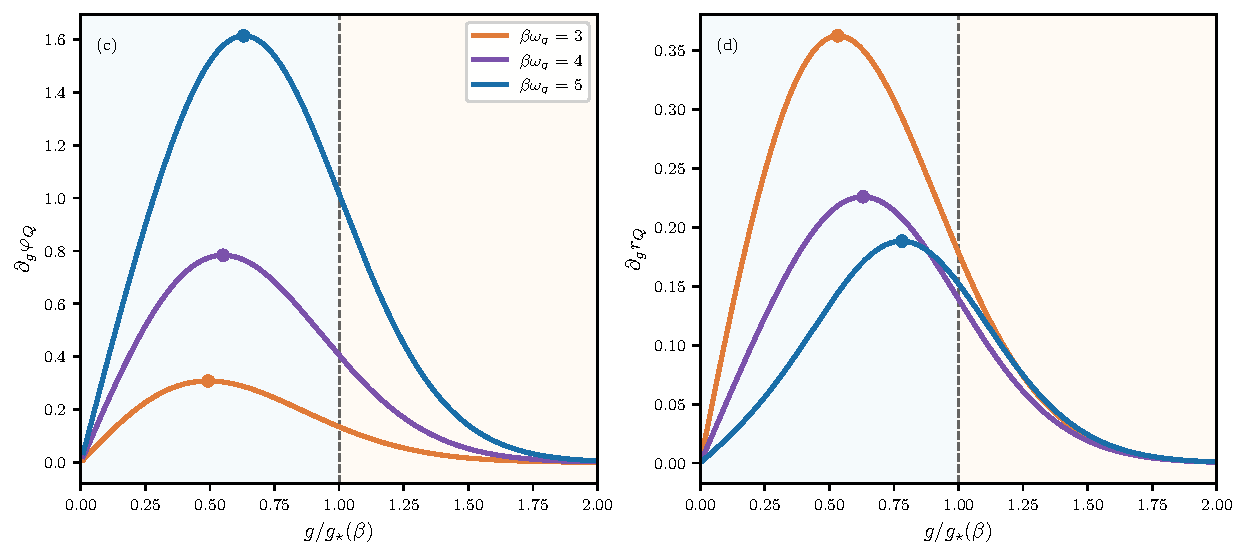
\includegraphics[width=\columnwidth]{../figures/hmf_fig1_chi_theory_cd_v3.pdf}
  \caption{Response susceptibilities of the exact reduced state.
    \textit{Panel~(c)}: Tilt susceptibility \(\partial_g\varphi_Q\) versus the
    scaled coupling \(g/g_\star(\beta)\).
    \textit{Panel~(d)}: Radius gradient \(\partial_g r_Q\) on the same scale.
    In both cases the peak positions collapse across temperatures and sit near,
    but not exactly on, the crossover line. The exact reduced state is therefore
    most sensitive to bath dressing in a narrow band around \(\chi\sim 1\).}
  \label{fig:chi_susceptibility}
\end{figure}

These figures do two jobs for the remainder of the paper. First, they make the
exact-state geometry visible: crossover, purification, and susceptibility are
all controlled by the same scalar response coordinate. Second, they identify
the narrow region where a compact reduced generator changes most rapidly. That
is precisely the region where finite-basis numerics become the hardest to keep
inside a restricted representational class.
